\subsection*{Cornelia}
Below is map of Cornelia, but there are also farms and smaller buildings outside the city walls that are not shown.
All buildings are marked with a number and you can find more details about them in the accordingly numbered paragraphs.
The party arrives in Cornelia from the southern gate, where two guards stop them as they do not recognize the adventurers.
They advise the party to stay clear of the castle and leave the town after finishing their business.
Most townspeople are too scared to leave their homes since the princess has disappeared.
\begin{center} 
	\tcbox[left=0pt,top=0pt,right=0pt,bottom=0pt, boxsep=0pt, colframe=accent, sharp corners]{
	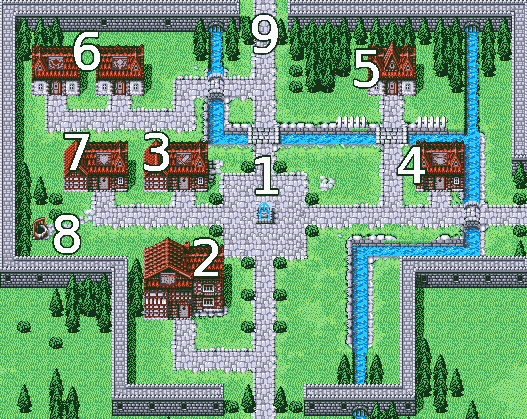
\includegraphics[width=0.98\columnwidth]{./art/maps/cornelia.png} 
	}
\end{center}
\subsubsection*{1. Fountain}
"Hello, there! I'm a dancer! What's that? You fancy a dance? Hee hee!"
-- Arylon \\ \\
The party notices a beautiful fountain standing out in the otherwise unremarkable town.
Nearby is a blue-haired cheerful young woman in a red dress who practices dancing, her name is Arylon.
When asked about the princess or the castle, she reveals rumors that she has heard: princess Sarah is being held hostage for a hefty ransom!
Accordingly, the castle is in chaos and has been locked off to regular folk.
She also reveals that there have been multiple unsuccessful attempts at rescuing Sarah.
She notices the weapons on the party and asks if they would be interested in helping.
 
\subsubsection*{2. Inn}
"Please, come in! We charge 50 Gil per night. Would you like to stay?"
-- Elia \\\\
The party enters into a small room with a red rug on the ground and a counter at its end.
Behind the counter stands a young woman with dark blue hair wearing a long green dress, her name is Elia.
To the left is a large room with multiple beds and minor decorations on the walls where the guests sleep.
To the right is another room, with wooden chairs and tables where guests can sit to eat and drink.
There is usually an old drunk man sitting there named Argus and sometimes also a few guards.
The party can sleep at the Inn for 50 Gil per night per person.  
They can also ask Elia for information, as she overhears a lot from visitors.
She points the party towards various people in town that may need their help such as the smith and the mages.  
The party can also speak to Argus, who babbles stories about a great soldier named Garland who he used to know from when he was a guard. 
 
\subsubsection*{3. Smith}
The party enters a large shop with a forge, where many weapons and armor are being displayed
Behind the counter is an older man with brown hair and a full beard, his name is Todo.
He informs the party that the store is closed, he cannot work due to not receiving essential shipments from the port.
To help him, the party has to talk to Dyce at Cornelia Port, who is looking after the shipments. 
They consist of a large wooden box on a small wagon, which slightly slows down the partys' movement.
On their way back, a bizarre monster named PuPu makes an attempt to steal the shipments!
PuPu is sitting in the trees, and uses his "Abduct" ability to slowly make the box disappear. 
If the players look for him in the trees while he is doing this, he is easy to spot, because the top of his head is glowing.
After that, he is difficult to spot, a player has to succeed on a check that can vary between DC 6-8.
The party may fail to find PuPu, but he will be nearby if they return to the same spot at a later time.
If detected, PuPu does not fight, he instead asks for Potions (see "Potions~Please!") and returns the stolen goods if the party complies.
You can also reward the party for solving the dispute peacefully, PuPu may for example return additional items or Gil.
The party can also just attack him, in which case the shipment reappears after PuPu is defeated.
Upon successfully bringing back the shipments, Todo rewards the party with 500 Gil.
The smith can start working again, but he will be busy completing outstanding orders for some time.
When the party returns in a few days, Todo may upgrade their weapons or armor and he may sell any Level 1 weapon or armor of your choice.
\vfill
\friendly{PuPu}{???}{
\includegraphics[width=0.13\textwidth]{./art/monsters/pupu.png}}
{
	HP: & \hfill 10 & MP: & \hfill 10\\
	STR: & \hfill 0 & DEF: & \hfill 0 \\
	MAG: & \hfill 0 & RES: & \hfill 0 \\
	AGI: & \hfill 2 & Size: & \hfill S\\
}
{
	\textbf{Drops}: All abducted objects 
	
	\mtech{Abduct}{0}{1r}{Single}{5u}{
		An object that you can see within range disappears to an unknown location.  
	}{}	
	\mpassive{Potion Please!}{
		Ask your enemies to give you a \hyperlink{item}{Potion}, if they comply make a DC 8 check.
		If you succeed you disappear to an unknown location (\hyperlink{status}{KO}), otherwise you keep asking for more \hyperlink{item}{Potions}.
	}
}

\subsubsection*{4. Store}
This general goods store is dominated by a large counter in the center and heaps of wares and items around it.
Behind the counter is a young man with dark hair and a green bandana, his name is Guston.
He is not particularly concerned about the princess, but he is annoyed that the troubles in Cornelia have dampened his sales.
Accordingly, he is very friendly towards potential customers and sells the items listed below.
He can have any other item of your choice in his inventory in addition.
\vspace{0.3cm}
\consumables{Items}{item2.png}{
	\hline Potion 		& 100 Gil & Regain 2d HP.  \\ 
	\hline Phoenix Down & 250 Gil & Remove \hyperlink{status}{KO} status and regain 1 HP.\\ 
	\hline Tent 		& 500 Gil & Allows the party to sleep outside. \\
	\hline Lantern 		& 100 Gil & A normal lantern.  \\ 
} 
 
\subsubsection*{5. Chapel}
"Do not lose heart, brave warriors."
\indent -- Gregory\\\\
The chapel is small and cozy with few wooden banks, but it is also completely empty except for one person, father Gregory.
Gregory is an old man with a long white beard wearing a red hooded robe, he speaks very slowly and quietly.
He laments that noone has been visiting the chapel since the disappearance of Sarah.
Apparently, most townspeople believe that the incident is a divine punishment, so they stay away from the chapel.
The father asks the party to restore the faith of Cornelia's citizen to fill the chapel again.
The party can for example convince people by clarifying details about Sarah's disappearance (she was kidnapped) that many are unaware of as the castle has been secretive.
If the party manages to convince at least any 3 people in Cornelia to attend the chapel, Gregory is satisfied and rewards them with 500~Gil.
Moreover, he offers his services to the party for free: he can cure cure the \hyperlink{status}{KO} status by performing a 1 hour long ritual. 

\subsubsection*{6. The Mages}
These two buildings are almost identical, each one consists of a single large room with a bed and shelves with heaps of magic and alchemy goods and books.
They are inhabited by the eccentric and stubborn twin brothers Gilles and Noah. 
Gilles is a Black Mage who wears a blue robe and a pointed hat, while Noah is a White Mage who wears a white hooded robe with red accents.
The other townspeople usually avoid the brothers, except when they need their services.
Getting annoyed by this, the mages have decided to develop a flask, which allows them store their magic inside, which others can use without their presence.
Unfortunately, something went wrong during its development, causing the item to break apart in a violent explosion, the result of which the party can see in the back yard.
Out of pride, both of them give blame their brother for the accident and they have stopped talking since.
The party can resolve the dispute by convincing them that they were both at fault.
They can for example achieve this as follows:
First they have to repair the broken flask either through mechanical or magical means, which is easy.
Then, they have to study the flask and the recipe for creating it, which they can get from the mages.
By doing this, a character that can use magic himself understands the issue, one that cannot use magic has to pass a DC 8 check.
The flask broke because after its creation, each mage cast 2 spells into it, causing the flask overload as it can only hold a total of 3 spells at most.
This can be demonstrated by casting only 3 spells into the flask, which works fine.
If the party manages to convince the mages, they accept their wrongdoing and apologize to each other.
They gift the flask to the party as a token of gratitude and the party may visit them in the future to buy the accessories shown below, to which you may add any other of your choice.
\vspace{0.3cm}
\accessory{Accessories}{acc.png}{
	\hline Magic Flask & 1000 Gil & Can store up to 3 spells that are cast into it. The wearer can use an action to unleash a stored spell's effect on a chosen target. \\ 
	\hline Rune \newline Bracers & 500 Gil & RES +1 \\
	\hline Mythril Shield & 500 Gil & DEF +1  \\ 
} 

\subsubsection*{7. Abandoned Building}
This building has been left purposefully empty in case you may need it.
It may for example related to one of the character's backgrounds or it may have content or characters that you want to add to the adventure.
If you have no use for it, the house is empty and the players can ask around the town to find out that it used to be a shop that has been abandoned due to not being profitable.
%If the party manages to bring back the princess safely, the king could also gift them this house as a reward.
%It will be very useful if the party will return to Cornelia in the future, otherwise they can try to sell it to someone.

\subsubsection*{8. Well}
It's a well. It looks like you could climb down it, but you can't. Really.

\subsubsection*{9. Castle Entrance}
This entrance directly leads to Castle Cornelia and is guarded by at least 4 guards day and night who do not let anyone pass.
However, they let the adventurers through if they explain that they want to help find the princess.
The guards then ask the party to report to the chancellor on the upper floor for further information.